\section{Cenário de Teste 4}

Este cenário está dividido em 5 (cinco) exemplos, os quais são apresentados a seguir, contemplando todo o processo de auto-localização
em cada exemplo, a partir da apresentação das Imagens abaixo.

\subsection{Exemplo 1}

{\centering
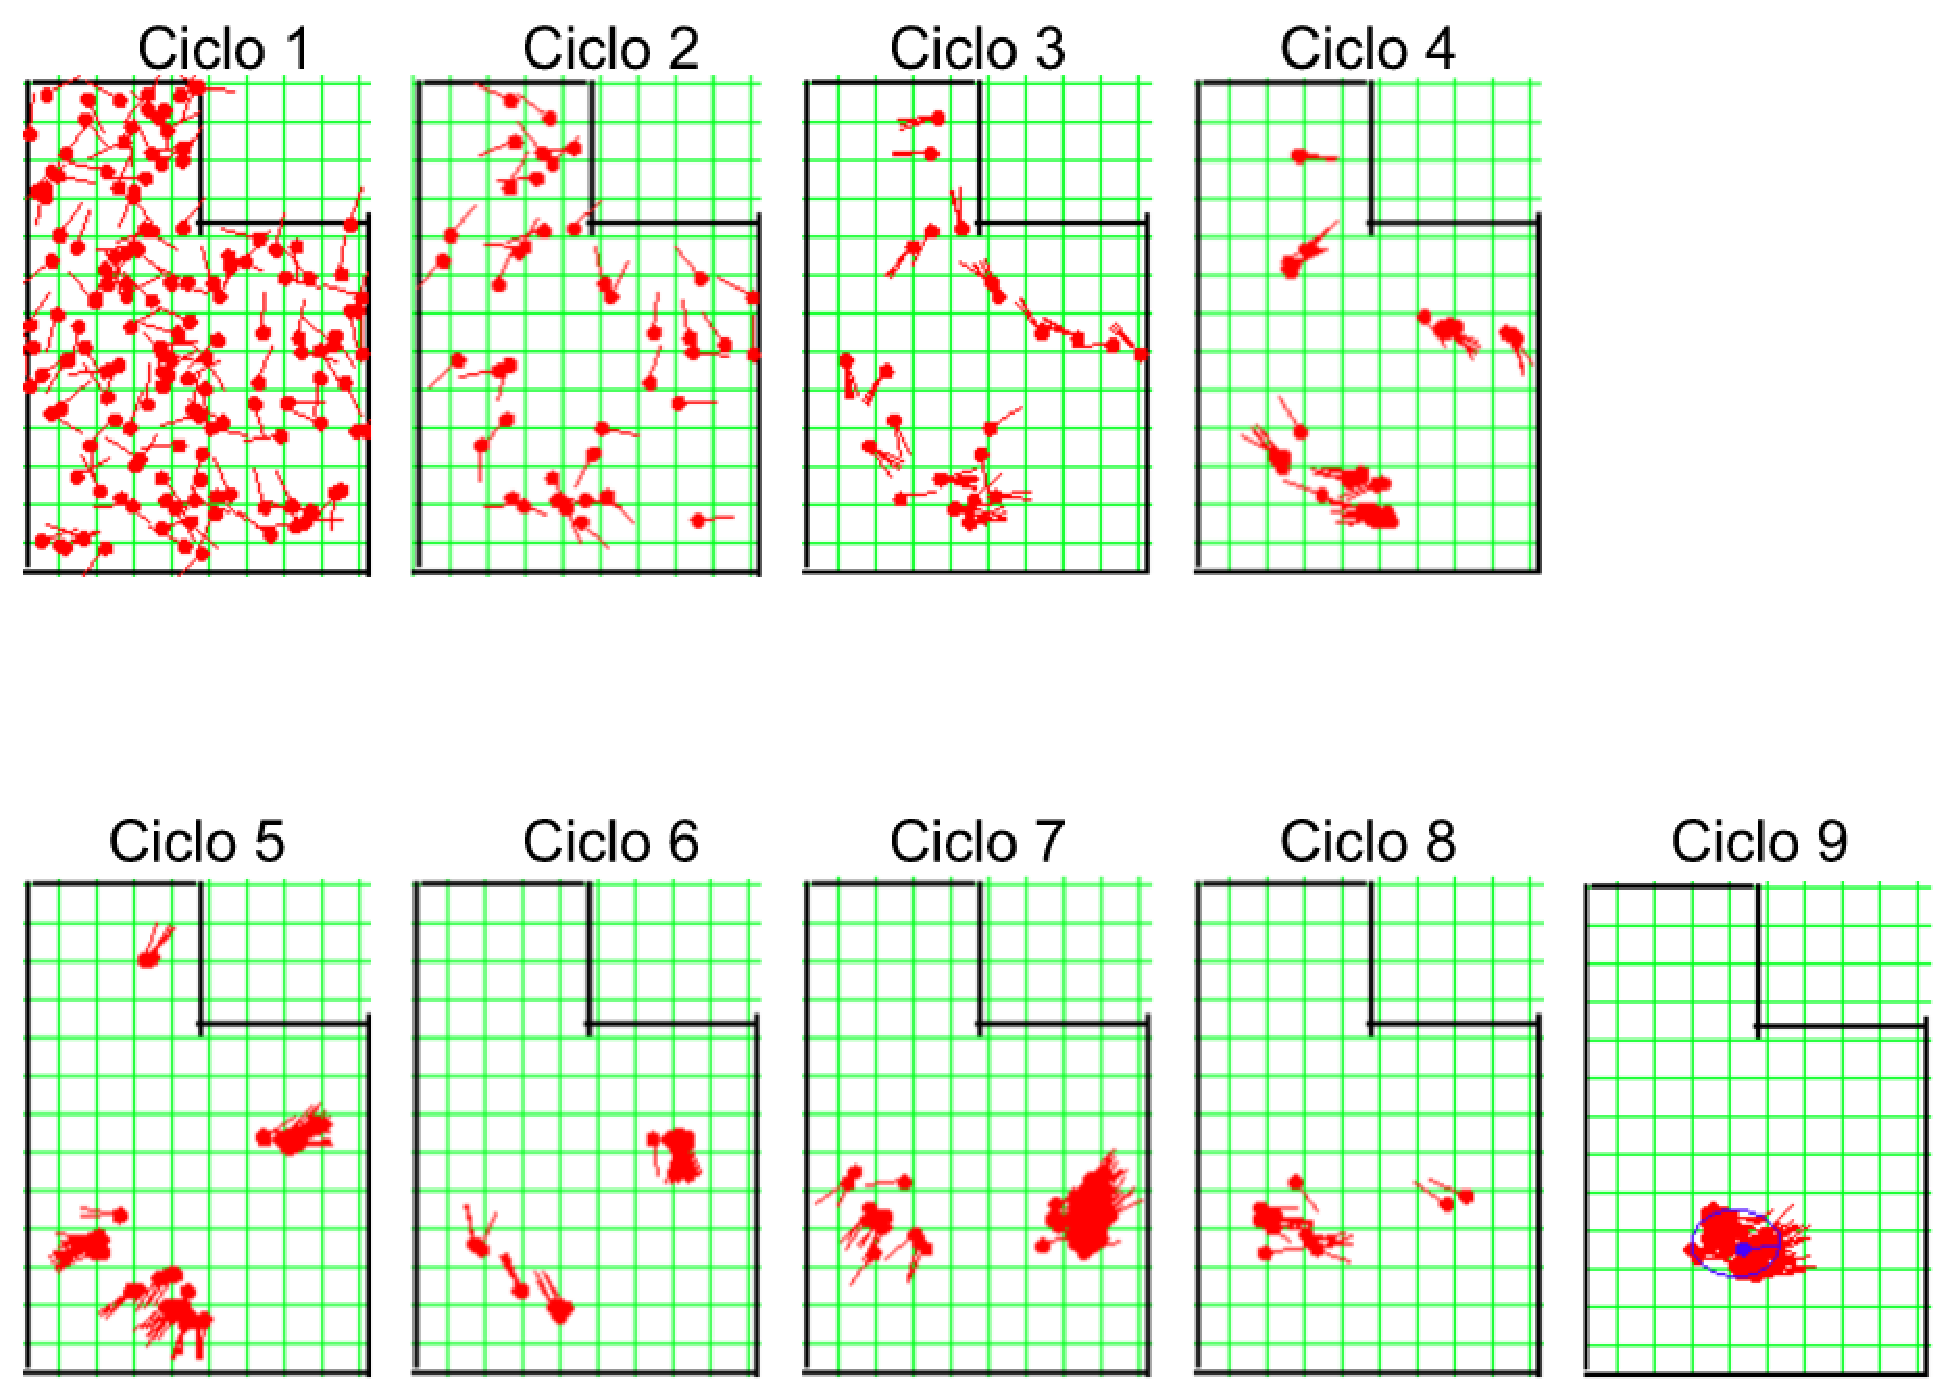
\includegraphics[scale=0.4]{figuras/cen4_ex1.eps}
\captionof{figure}{Cenário 4 - Exemplo 1}
\label{img:cen4_ex1}
\par}

{\centering
\includegraphics[scale=0.2]{figuras/real_cen4_ex1.eps}
\captionof{figure}{Posição Real do Cenário 4 - Exemplo 1.}
\label{img:real_cen4_ex1}
\par}

\subsection{Exemplo 2}

{\centering
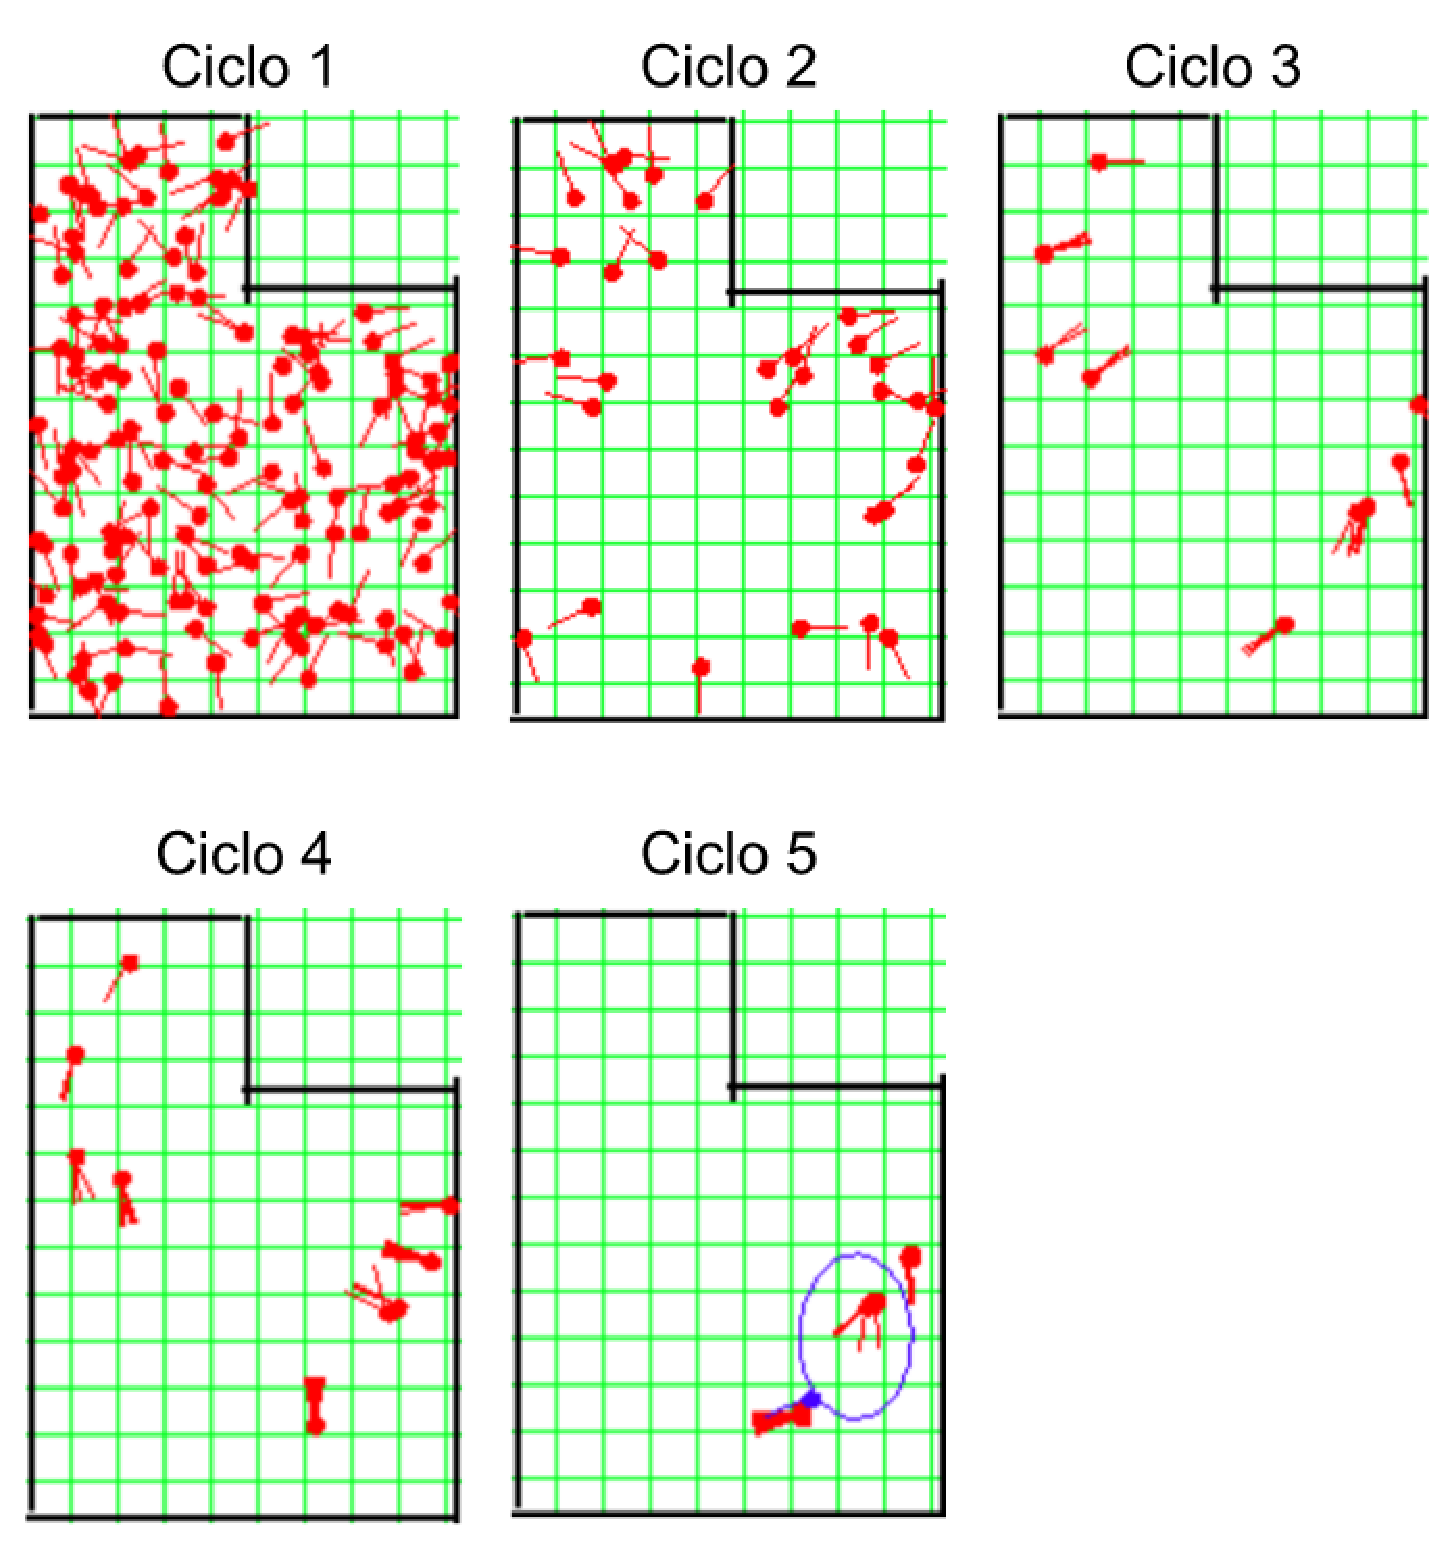
\includegraphics[scale=0.4]{figuras/cen4_ex2.eps}
\captionof{figure}{Cenário 4 - Exemplo 2}
\label{img:cen4_ex2}
\par}

{\centering
\includegraphics[scale=0.2]{figuras/real_cen4_ex2.eps}
\captionof{figure}{Posição Real do Cenário 4 - Exemplo 2.}
\label{img:real_cen4_ex2}
\par}

\subsection{Exemplo 3}

{\centering
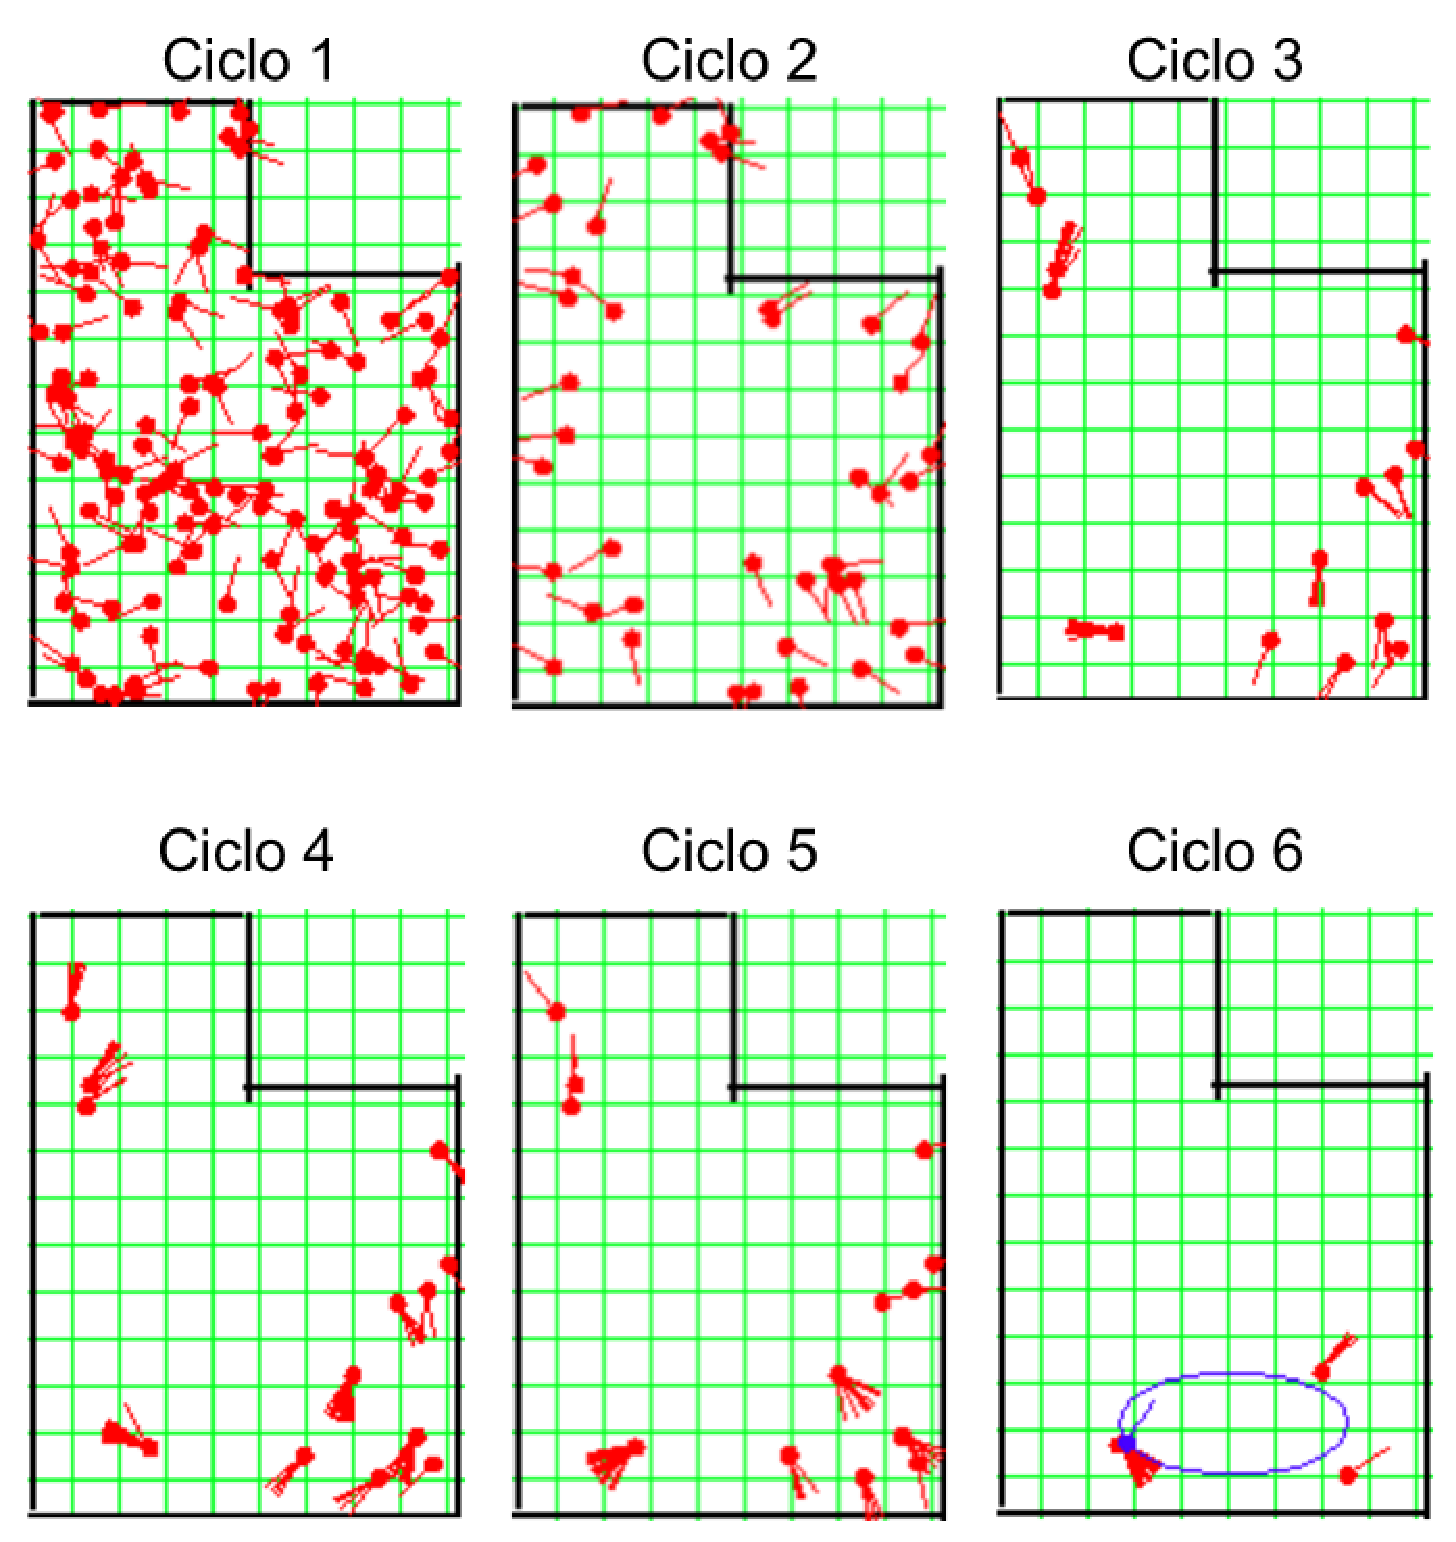
\includegraphics[scale=0.4]{figuras/cen4_ex3.eps}
\captionof{figure}{Cenário 4 - Exemplo 3}
\label{img:cen4_ex3}
\par}

{\centering
\includegraphics[scale=0.2]{figuras/real_cen4_ex3.eps}
\captionof{figure}{Posição Real do Cenário 4 - Exemplo 3.}
\label{img:real_cen4_ex3}
\par}

\subsection{Exemplo 4}

{\centering
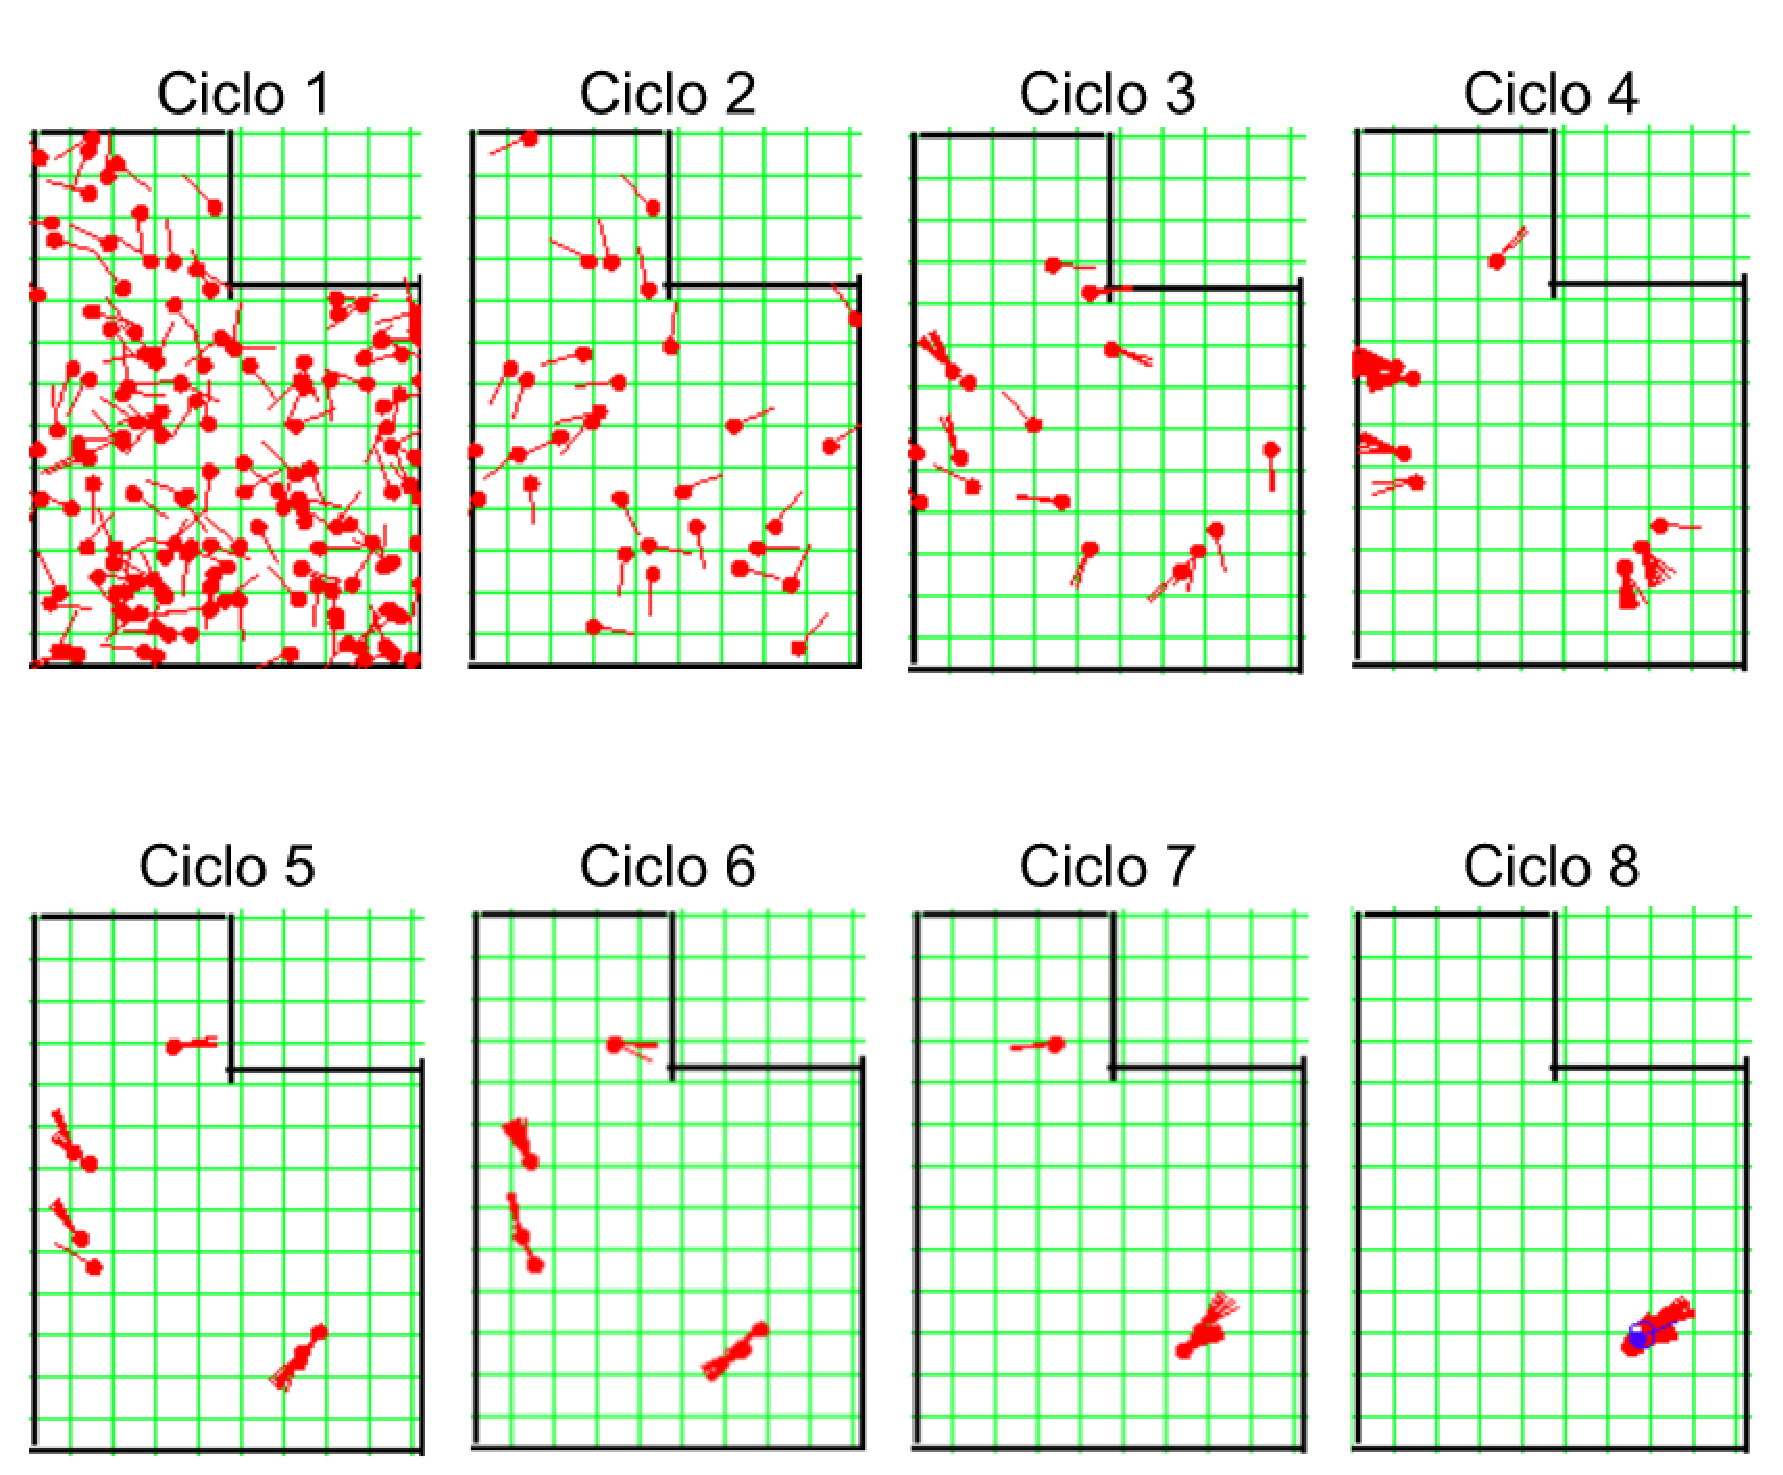
\includegraphics[scale=0.4]{figuras/cen4_ex4.eps}
\captionof{figure}{Cenário 4 - Exemplo 4}
\label{img:cen4_ex4}
\par}

{\centering
\includegraphics[scale=0.2]{figuras/real_cen4_ex4.eps}
\captionof{figure}{Posição Real do Cenário 4 - Exemplo 4.}
\label{img:real_cen4_ex4}
\par}

\subsection{Exemplo 5}

{\centering
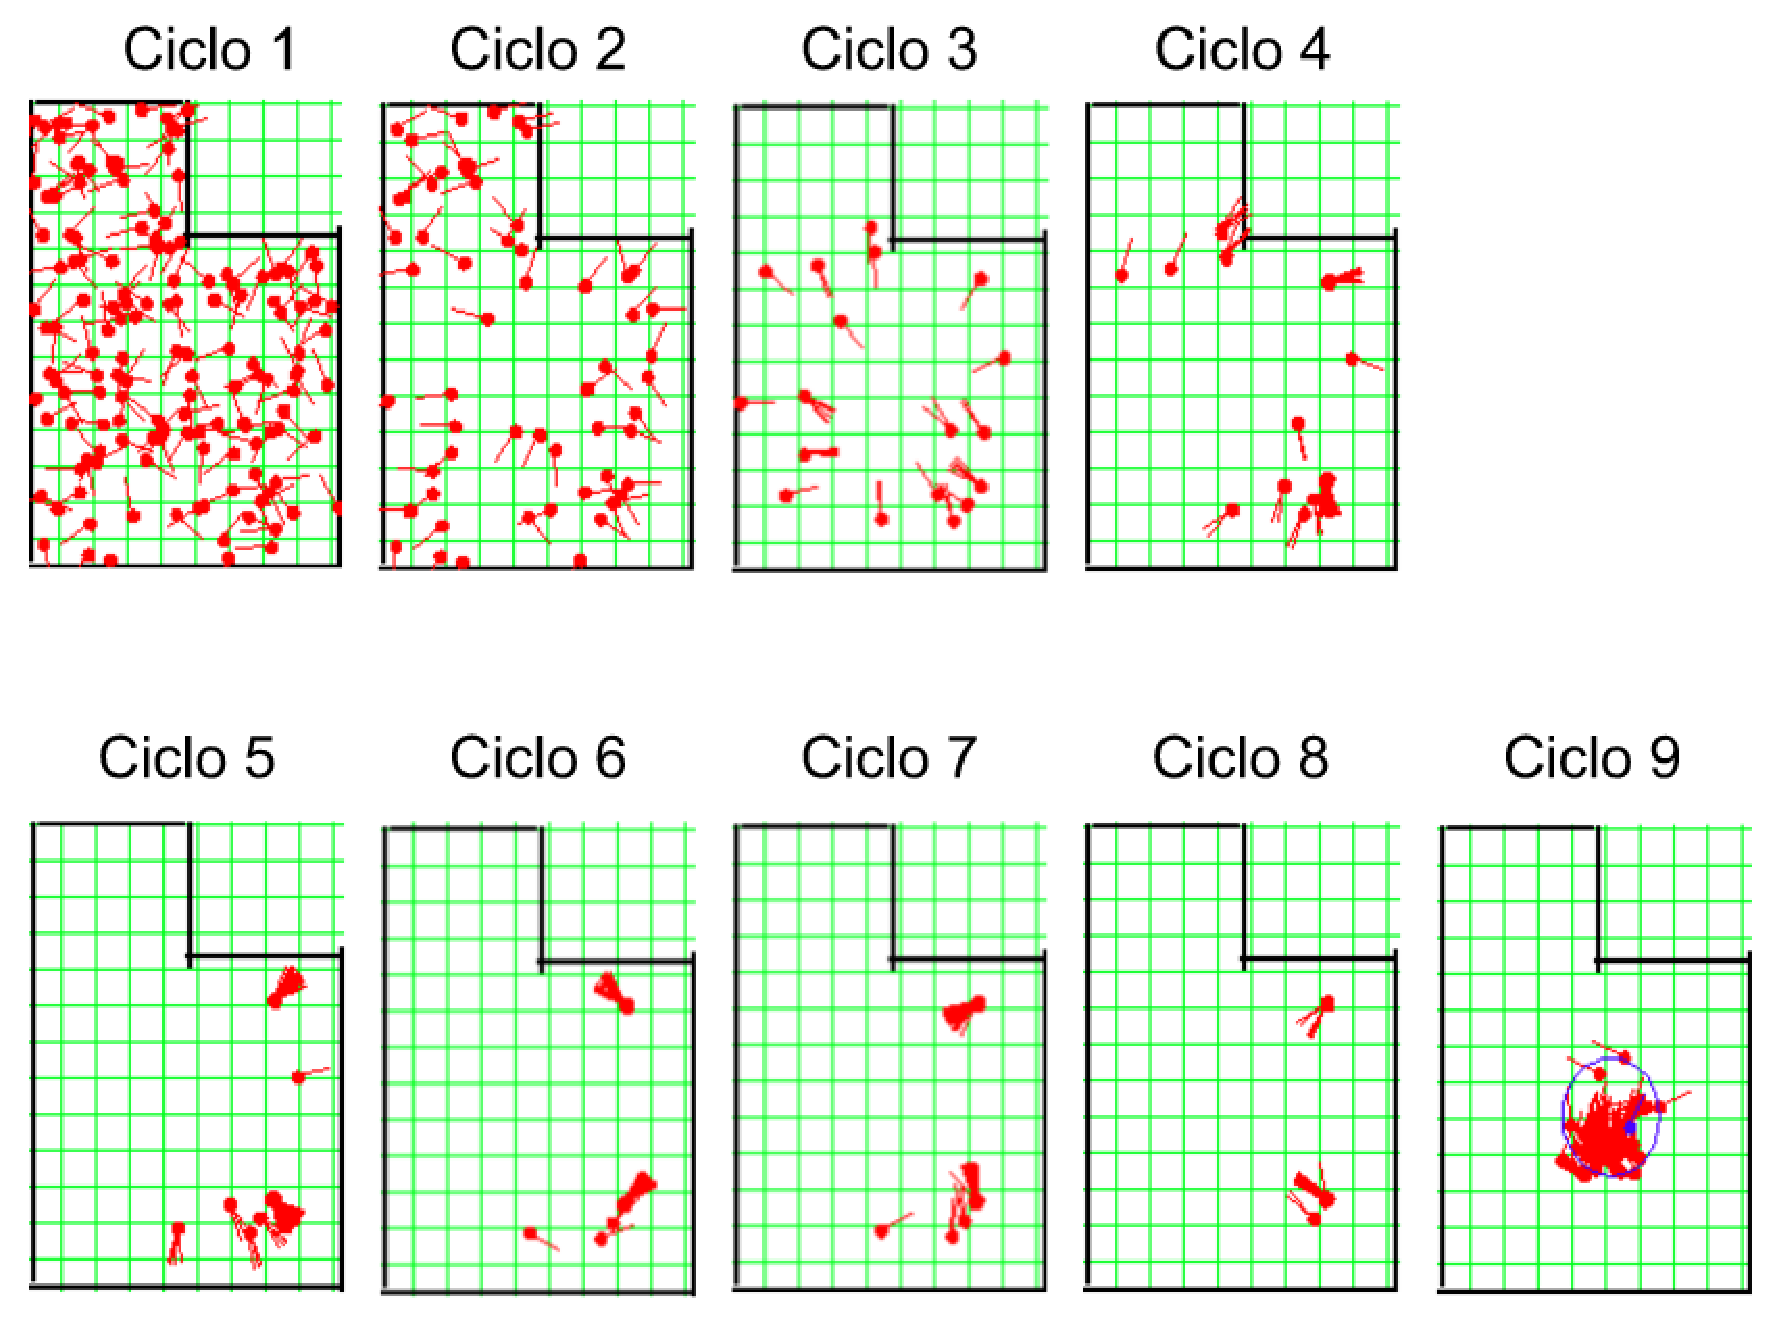
\includegraphics[scale=0.4]{figuras/cen4_ex5.eps}
\captionof{figure}{Cenário 4 - Exemplo 5}
\label{img:cen4_ex5}
\par}

{\centering
\includegraphics[scale=0.2]{figuras/real_cen4_ex5.eps}
\captionof{figure}{Posição Real do Cenário 4 - Exemplo 5.}
\label{img:real_cen4_ex5}
\par}
